% ================================================================
\section{Algoritmos gulosos, matroides e árvores geradoras mínimas}\label{sec:gulosos}
% ================================================================

\subsection{Método guloso (slides de Matroides)}\label{sec:guloso}
\textbf{Esquema geral:} queremos $S'\subseteq S$ que satisfaça uma propriedade $P$ e seja máximo (ou mínimo) por um critério. O guloso começa com $S'_0=\emptyset$ e, a cada passo, acrescenta o elemento $s$ que mantém $P$ e é o \textbf{melhor segundo o critério naquele momento}, sem nunca desfazer escolhas. Para enquanto houver tal $s$.
\begin{itemize}
  \item \textbf{Quando dá o ótimo?} Quando vale a \textbf{propriedade gulosa}: existe uma solução ótima que contém o elemento escolhido, e, fixado esse elemento, resta resolver um subproblema bem definido do mesmo tipo (subestrutura ótima).
  \item \textbf{Como provar:} \emph{argumento de troca}. Tome uma ótima $O$ que concorde com o guloso o máximo possível; no primeiro ponto de discordância, troque um elemento de $O$ pelo do guloso sem piorar. Isso contradiz a escolha de $O$, ou mostra que o guloso também é ótimo.
  \item \textbf{O que os problemas gulosos têm em comum?} Em grande parte deles o sistema de conjuntos viáveis é uma \textbf{matroide} (§\ref{sec:matroides}).
  \item \textbf{PD $\times$ guloso:} a PD testa todas as escolhas de cada subproblema (tabela); o guloso faz uma escolha só e nunca volta atrás. É mais rápido, mas só funciona com a propriedade gulosa.
\end{itemize}

\begin{pseudo}{Troco guloso (lista de AGM e gulosos, ex.~8)}
\begin{algorithmic}
\Function{TrocoGuloso}{$S,\ v_1>v_2>\dots>v_n$} \Comment{moedas em ordem decrescente}
  \State $total:=0$
  \For{$i:=1$ \textbf{até} $n$}
    \State $q_i:=\floor{S/v_i}$;\ $S:=S-q_i\,v_i$;\ $total:=total+q_i$ \Comment{o máximo possível da maior moeda}
  \EndFor
  \State \Return $total$ \Comment{se $S\ne0$ ao final, não há troco exato}
\EndFunction
\end{algorithmic}
\end{pseudo}
\textbf{Ótimo para $\{10,5,2,1\}$.} Seja $(a,b,c,d)$ o número de moedas de $10,5,2,1$ numa solução ótima. Então $d\le1$ (duas de 1 viram uma de 2), $b\le1$ (duas de 5 viram uma de 10), $c\le2$ (três de 2 viram $5+1$) e não ocorre $c=2$ com $d=1$ ($2+2+1$ vira uma de 5). Logo as moedas pequenas somam $5b+2c+d\le9<10$, e então $a=\floor{S/10}$, como no guloso. Do mesmo modo, $2c+d\le4<5$ força $b$ igual ao do guloso, e $d\le1$ força $c$. A ótima \emph{é} a gulosa (conferido para $S\le500$).
\textbf{Não funciona sempre:} $\{4,3,1\}$ com $S=6$: o guloso dá $4+1+1$ (3 moedas), mas $3+3$ usa 2. Outro: $\{25,10,1\}$ com $S=30$: guloso 6 moedas, ótimo $10+10+10$. (O caso geral se resolve por PD, como a mochila ilimitada: $T(s)=1+\min_{v_i\le s}T(s-v_i)$, em $\Theta(nS)$.)

% ------------------------------------------------------------------
\subsection{Matroides (slides de Matroides; pesquisa)}\label{sec:matroides}
\begin{defi}[Matroide; Whitney, 1935]
$M=(E,\mathcal I)$, com $E$ finito e $\mathcal I\subseteq2^E$ (os \textbf{independentes}), tal que:
(I1) $\emptyset\in\mathcal I$;\quad
(I2) se $I\in\mathcal I$ e $I'\subseteq I$, então $I'\in\mathcal I$ (\emph{sistema de subconjuntos}, fechado para baixo);\quad
(I3) se $I_1,I_2\in\mathcal I$ e $|I_1|<|I_2|$, existe $e\in I_2\setminus I_1$ com $I_1\cup\{e\}\in\mathcal I$ (\textbf{aumento}, ou troca).
\end{defi}
O modelo é a independência linear: ``independente'' generaliza ``linearmente independente'' (matrizes) e ``acíclico'' (grafos).
\begin{center}\small
\begin{tabularx}{\linewidth}{@{}lX@{}}
\toprule
Matroide & Independentes\\
\midrule
\textbf{Linear} & conjuntos de colunas (vetores) de uma matriz linearmente independentes.\\
\textbf{Gráfica} (de $G$) & conjuntos de arestas \textbf{acíclicos} (florestas). Bases $=$ árvores geradoras (se $G$ é conexo).\\
\textbf{Uniforme} $U_{n,k}$ & todos os $I\subseteq E$ com $|I|\le k$ (\emph{livre} se $k=n$).\\
\textbf{Partição} & $E=E_1\cup\dots\cup E_t$ (partição) e $I$ com $|I\cap E_i|\le k_i$ para todo $i$.\\
\textbf{Transversal} & em $G$ bipartido $(X,Y)$: os $I\subseteq X$ \emph{emparelháveis} (cobertos por algum emparelhamento).\\
\textbf{Emparelhamento} & em $G$ qualquer: os $I\subseteq V$ cobertos por algum emparelhamento.\\
\textbf{Dual} $M^*$ & bases são os complementos $E\setminus B$ das bases de $M$ (dual da gráfica: \emph{cográfica}).\\
\bottomrule
\end{tabularx}
\end{center}
\textbf{(I3) para a gráfica} (exercício dos slides): uma floresta com $k$ arestas em $n$ vértices tem $n-k$ componentes. Como $|I_1|<|I_2|$, $I_2$ tem menos componentes que $I_1$, então alguma aresta $e\in I_2$ liga duas componentes diferentes de $I_1$ (se todas as arestas de $I_2$ ficassem dentro de componentes de $I_1$, cada componente de $I_2$ caberia numa de $I_1$, e $I_2$ teria pelo menos tantas componentes quanto $I_1$). Logo $I_1\cup\{e\}$ é acíclico.
\textbf{(I3) para a linear}: $\operatorname{span}(I_1)$ tem dimensão $|I_1|<|I_2|$, então algum vetor de $I_2$ está fora dele, e acrescentá-lo a $I_1$ mantém a independência.

\paragraph{Formas equivalentes de (I3) e bases.}
\begin{itemize}
  \item \textbf{(I3$'$)} Para todo $X\subseteq E$, todos os independentes \emph{maximais} contidos em $X$ têm o mesmo tamanho (o \textbf{posto} $r(X)$). [$\Rightarrow$: se $|I_1|<|I_2|$ maximais em $X$, (I3) aumentaria $I_1$ dentro de $X$. $\Leftarrow$: em $X=I_1\cup I_2$, estenda $I_1$ a um maximal $B_1$; como $|B_1|\ge|I_2|>|I_1|$, existe $e\in B_1\setminus I_1\subseteq I_2\setminus I_1$, e $I_1\cup\{e\}\subseteq B_1$ é independente por (I2).]
  \item \textbf{(I3$''$)} Todos os maximais de $\mathcal I$ têm o mesmo tamanho $r$, e se $|I|=r$, $|I'|=r-1$, existe $x\in I\setminus I'$ com $I'\cup\{x\}\in\mathcal I$.
  \item \textbf{Base}: independente maximal; todas têm o mesmo tamanho. A coleção $\mathcal B$ de bases satisfaz (B1) $\mathcal B\ne\emptyset$ e (B2) (\textbf{troca de bases}): se $B_1,B_2\in\mathcal B$ e $x\in B_1\setminus B_2$, existe $y\in B_2\setminus B_1$ com $(B_1\setminus\{x\})\cup\{y\}\in\mathcal B$. Reciprocamente, toda $\mathcal B$ com (B1)(B2) é a coleção de bases da matroide $\mathcal I=\{I:I\subseteq B\text{ para algum }B\in\mathcal B\}$.
\end{itemize}

\paragraph{Algoritmo guloso para matroides (base de peso máximo).} Dados $M$ e $c:E\to\R$, achar uma base de peso $c(B)=\sum_{e\in B}c(e)$ máximo. Os independentes são dados \emph{implicitamente}, por um \textbf{oráculo} que responde ``$X$ é independente?'' (listá-los pode ser exponencial).
\begin{pseudo}{GreedyAlgorithm$(M,c)$ (slides) -- $O(n\log n+n\,h)$, $h=$ custo do oráculo}
\begin{algorithmic}
\Function{Guloso}{$M,c$}
  \State $B:=\emptyset$
  \State ordene $E$: $c(e_1)\ge c(e_2)\ge\dots\ge c(e_n)$ \Comment{não crescente}
  \For{$i:=1$ \textbf{até} $n$}
    \If{$B\cup\{e_i\}$ é independente em $M$} \State $B:=B\cup\{e_i\}$ \EndIf
  \EndFor
  \State \Return $B$
\EndFunction
\end{algorithmic}
\end{pseudo}
\begin{teo}[Rado--Edmonds]\label{teo:gulosomat}
Se $M$ é matroide, \textup{\textsc{Guloso}} devolve uma base de peso máximo, para qualquer $c$.
\end{teo}
\emph{Prova (slides).} Seja $B$ a saída (é base, pois nada mais cabe) e $B^*$ uma base ótima com $|B\cap B^*|$ máximo. Se $B\ne B^*$, seja $f$ o primeiro elemento (na ordem do algoritmo) de $B\setminus B^*$; os escolhidos antes de $f$ formam $B'\subseteq B^*$. Pela troca de bases, existe $e\in B^*\setminus B$ com $(B^*\setminus\{e\})\cup\{f\}$ base. Pela otimalidade de $B^*$, $c(f)\le c(e)$. Se $c(f)=c(e)$, essa nova base seria ótima e teria mais elementos em comum com $B$: contradição. Logo $c(f)<c(e)$, e $e$ vem antes de $f$ na ordem. Mas quando $e$ foi examinado, o conjunto escolhido estava contido em $B'$, e $B'\cup\{e\}\subseteq B^*$ é independente: o algoritmo teria escolhido $e$. Contradição. $\square$

\textbf{A recíproca também vale} (definição alternativa): se $\mathcal I$ satisfaz (I1)(I2) e o guloso acerta para \emph{todo} $c$, então vale (I3). [Suponha $|I_1|=k<|I_2|$ e que nenhum $e\in I_2\setminus I_1$ aumente $I_1$. Use $c=k+2$ em $I_1$, $c=k+1$ em $I_2\setminus I_1$ e $c=0$ no resto. O guloso pega $I_1$ primeiro, não consegue pegar nada de $I_2\setminus I_1$ e termina com peso $k(k+2)$. Mas $I_2$ pesa pelo menos $(k+1)(k+1)>k(k+2)$. Contradição.] Ou seja, \textbf{matroides são exatamente os sistemas em que o guloso é sempre ótimo}.
\begin{itemize}
  \item \textbf{Base de peso mínimo}: ordem não decrescente (ou pesos $-c$). Kruskal é exatamente isso na matroide gráfica (§\ref{sec:kruskal}).
  \item \textbf{Testar se $k$ colunas de uma matriz $m\times k$ são LI} (``para praticar''): escalonamento (Gauss), $O(m\,k\min\{m,k\})$; se $k>m$, já são dependentes.
  \item \textbf{Escalonamento de intervalos} (pesos unitários): o guloso ``termina primeiro'' é ótimo, mas \textbf{não} é matroide. Com $I_1=\{[1,10]\}$ e $I_2=\{[1,2],[3,4]\}$, nenhum intervalo de $I_2$ cabe junto com $[1,10]$, e (I3) falha. A otimalidade vem de um argumento de troca específico; com pesos arbitrários o guloso falha e é preciso PD.
  \item \textbf{Emparelhamento} (conjuntos de arestas) num grafo qualquer \textbf{não} é matroide: no caminho $a\!-\!b\!-\!c\!-\!d$, $\{bc\}$ não pode ser aumentado por $ab$ nem por $cd$ (de $\{ab,cd\}$). Um guloso que pegue $bc$ primeiro fica com 1 aresta, e o máximo é 2.
\end{itemize}

\begin{complemento}[ -- pesquisa ``Matroides, algoritmos gulosos e generalizações polinomiais'']
\textbf{Interseção de matroides.} Dadas $M_1=(E,\mathcal I_1)$ e $M_2=(E,\mathcal I_2)$, achar $I\in\mathcal I_1\cap\mathcal I_2$ de tamanho (ou peso) máximo. Exemplos: \emph{emparelhamento bipartido} $=$ interseção de duas matroides de partição (no máximo uma aresta por vértice de $X$; idem para $Y$); \emph{floresta colorida} (exemplo 2 da pesquisa) $=$ gráfica $\cap$ partição pelas cores (no máximo uma aresta de cada cor); \emph{árvore geradora ``arco-íris''}.
\textbf{Por que o guloso falha} (exemplo 3): a interseção de duas matroides em geral não é matroide (o caminho $a\!-\!b\!-\!c\!-\!d$ acima é bipartido).
\textbf{Algoritmo (Edmonds/Lawler):} caminhos aumentantes num \emph{grafo de troca}. Dado $I$ comum, para $y\in I$ e $x\notin I$: arco $y\to x$ se $I-y+x\in\mathcal I_1$, e arco $x\to y$ se $I-y+x\in\mathcal I_2$. As fontes são os $x$ com $I+x\in\mathcal I_1$ e os destinos os $x$ com $I+x\in\mathcal I_2$. Um caminho \emph{mais curto} de uma fonte a um destino dá $I\,\triangle\,\text{caminho}$ comum com um elemento a mais; se não há caminho, $I$ é máximo. São $\le r$ aumentos, cada um com $O(nr)$ chamadas ao oráculo: \textbf{polinomial}. Vale o teorema min-max: $\max|I|=\min_{U\subseteq E}\{r_1(U)+r_2(E\setminus U)\}$.
\textbf{Três matroides: NP-difícil.} O \emph{caminho hamiltoniano} num digrafo é um independente comum de tamanho $n-1$ de três matroides: a gráfica do grafo subjacente (sem ciclos), a partição ``grau de entrada $\le1$'' e a partição ``grau de saída $\le1$''.
\textbf{Particionamento de matroides} (cobrir $E$ com o menor número de independentes; ex.: cobrir as arestas com o menor número de florestas, a \emph{arboricidade}) também é polinomial. Moral: reconhecer que um problema é interseção ou partição de matroides prova que ele é polinomial.
\end{complemento}

% ------------------------------------------------------------------
\subsection{Árvore geradora mínima (AGM)}\label{sec:agm}
\textbf{Problema:} dado $G$ conexo com pesos $c$ nas arestas, achar uma árvore geradora (conexa, acíclica, com os $n$ vértices e, portanto, $n-1$ arestas) de peso total mínimo. Os dois algoritmos são gulosos e a correção de ambos vem do lema abaixo.
\begin{lema}[Propriedade do corte; Cormen, Teo.~23.1]\label{lema:corte}
Seja $A$ um conjunto de arestas contido em alguma AGM, e $(S,V\setminus S)$ um corte que nenhuma aresta de $A$ atravessa. Se $e$ é uma aresta de peso mínimo entre as que atravessam o corte, então $A\cup\{e\}$ está contido em alguma AGM.
\end{lema}
\emph{Prova (troca).} Seja $T$ uma AGM com $A\subseteq T$. Se $e\in T$, acabou. Senão, $T+e$ tem um ciclo que passa por $e$; como $e$ atravessa o corte, o ciclo o atravessa de novo por outra aresta $f\in T$, com $f\notin A$. $T'=T+e-f$ é árvore geradora e $c(T')=c(T)+c(e)-c(f)\le c(T)$. Logo $T'$ é AGM e contém $A\cup\{e\}$. $\square$

\subsubsection{Algoritmo de Kruskal (aula 17, 09/10; slides 406--449; Cormen §23.2)}\label{sec:kruskal}
A solução parcial é uma \textbf{floresta}: percorre as arestas em ordem crescente de peso e aceita cada uma que \textbf{não forma ciclo}, isto é, que une duas árvores diferentes. O teste de ciclo usa conjuntos disjuntos (§\ref{sec:uf}).
\begin{pseudo}{Kruskal com Union-Find (slides, ``nova versão'')}
\begin{algorithmic}
\Function{Kruskal}{$G,c$}
  \State $E(T):=\emptyset$
  \For{\textbf{cada} $v\in V$} \State \MakeSet$(v)$ \Comment{$n$ árvores triviais} \EndFor
  \State ordene as arestas: $c(e_1)\le c(e_2)\le\dots\le c(e_m)$ \Comment{$O(m\log m)=O(m\log n)$}
  \For{$j:=1$ \textbf{até} $m$}
    \State seja $e_j=uv$
    \If{\Find$(u)\ne$ \Find$(v)$} \Comment{une duas árvores distintas: não fecha ciclo}
      \State $E(T):=E(T)\cup\{e_j\}$;\ \Union$(u,v)$
    \EndIf
  \EndFor
  \State \Return $T$ \Comment{pode parar quando $|E(T)|=n-1$}
\EndFunction
\end{algorithmic}
\end{pseudo}
\textbf{Complexidade:} a ordenação domina, $O(m\log m)=O(m\log n)$, porque $m\le n^2$ dá $\log m\le2\log n$. O laço custa $O(m+n\log n)$ com listas e união ``menor na maior'' (slides: cada vértice muda de conjunto no máximo $\log n$ vezes), ou $O(m\,\alpha(n))$ com floresta, rank e compressão. \textbf{Total: $O(m\log n)$.}
\textbf{Correção:} ao aceitar $e=uv$, tome $S=$ árvore atual de $u$. Nenhuma aresta aceita atravessa esse corte, e $e$ é a mais leve que o atravessa: uma mais leve teria sido examinada antes, quando seus extremos já estavam em árvores diferentes (as árvores só crescem), e teria sido aceita. Pelo Lema~\ref{lema:corte}, segue por indução. (Também é o Teorema~\ref{teo:gulosomat} aplicado à matroide gráfica.)

\begin{center}
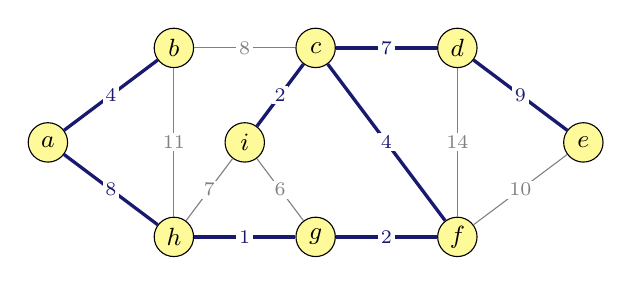
\begin{tikzpicture}[v/.style={circle,draw,fill=yellow!40,inner sep=1.2pt,minimum size=5mm,font=\small},
  agm/.style={very thick,MidnightBlue}, nao/.style={thin,gray}, w/.style={font=\scriptsize,fill=white,inner sep=1pt}]
\node[v] (a) at (0,1.2) {$a$}; \node[v] (b) at (1.6,2.4) {$b$}; \node[v] (c) at (3.4,2.4) {$c$}; \node[v] (d) at (5.2,2.4) {$d$};
\node[v] (e) at (6.8,1.2) {$e$}; \node[v] (f) at (5.2,0) {$f$}; \node[v] (g) at (3.4,0) {$g$}; \node[v] (h) at (1.6,0) {$h$};
\node[v] (i) at (2.5,1.2) {$i$};
\draw[agm] (a)--node[w]{4}(b); \draw[agm] (a)--node[w]{8}(h); \draw[nao] (b)--node[w]{11}(h); \draw[nao] (b)--node[w]{8}(c);
\draw[nao] (h)--node[w]{7}(i); \draw[agm] (h)--node[w]{1}(g); \draw[agm] (i)--node[w]{2}(c); \draw[nao] (i)--node[w]{6}(g);
\draw[agm] (c)--node[w]{7}(d); \draw[agm] (c)--node[w]{4}(f); \draw[agm] (g)--node[w]{2}(f); \draw[nao] (d)--node[w]{14}(f);
\draw[agm] (d)--node[w]{9}(e); \draw[nao] (e)--node[w]{10}(f);
\end{tikzpicture}
\end{center}
\begin{exemplo}[Grafo dos slides (Cormen, Fig.~23.4) --- conferido]
\textbf{Kruskal} aceita $hg(1)$, $ic(2)$, $gf(2)$, $ab(4)$, $cf(4)$, $cd(7)$, $ah(8)$, $de(9)$ e rejeita $ig(6)$, $hi(7)$, $bc(8)$, $ef(10)$, $bh(11)$, $df(14)$, que fechariam ciclo. \textbf{Custo 37} (azul).
\textbf{Prim} com raiz $a$ acrescenta $ab(4)$, $ah(8)$, $hg(1)$, $gf(2)$, $fc(4)$, $ci(2)$, $cd(7)$, $de(9)$: mesma árvore, custo 37. \emph{A AGM não é única}: $ah$ e $bc$ pesam 8, e trocar uma pela outra dá outra AGM de custo 37 (é a que aparece no Cormen). Com pesos todos distintos, a AGM é única.
\end{exemplo}

\subsubsection{Algoritmo de Prim (aula 17; slides 450--461 e slide de AGM)}\label{sec:prim}
A solução parcial é uma \textbf{árvore} que cresce a partir de uma raiz: a cada passo entra a aresta mais leve com um extremo em $V(T)$ e o outro fora. \textbf{Correção:} Lema~\ref{lema:corte} com $S=V(T)$.
\begin{pseudo}{Prim em $O(n^2)$ com vetores (lista, ex.~4 e 5)}
\begin{algorithmic}
\Function{Prim}{$G,W,r$}
  \State para todo $v$: $chave(v):=\infty$;\ $pai(v):=\nil$;\ $dentro(v):=$ falso
  \State $chave(r):=0$
  \For{$it:=1$ \textbf{até} $n$}
    \State $u:=$ vértice com $dentro(u)=$ falso e $chave(u)$ mínima \Comment{varredura: $O(n)$}
    \State $dentro(u):=$ verdadeiro \Comment{se $u\ne r$, a aresta $pai(u)\,u$ entra em $T$}
    \For{\textbf{cada} $v\in N(u)$ com $dentro(v)=$ falso} \Comment{matriz: linha $u$, $O(n)$; listas: $O(\text{grau}(u))$}
      \If{$W(u,v)<chave(v)$} \State $chave(v):=W(u,v)$;\ $pai(v):=u$ \EndIf
    \EndFor
  \EndFor
  \State \Return $\{\,pai(v)\,v : v\ne r\,\}$
\EndFunction
\end{algorithmic}
\end{pseudo}
$chave(v)$ é o peso da aresta mais leve de $v$ até a árvore. É o mesmo esqueleto do Dijkstra, trocando ``$L(u)+W(u,v)$'' por ``$W(u,v)$''.
\begin{center}\small
\begin{tabular}{@{}lll@{}}
\toprule
Implementação & Custo & Comentário\\
\midrule
Matriz de adjacência + vetor $chave$ & $O(n^2)$ & $n$ varreduras de $O(n)$; ótimo para matriz\\
Listas de adjacência + vetor $chave$ & $O(n^2+m)=O(n^2)$ & a varredura domina\\
Listas + heap binário (\emph{decrease-key}) & $O(m\log n)$ & $n$ remoções $+$ $\le m$ reduções, $O(\log n)$ cada\\
Listas + heap de Fibonacci & $O(m+n\log n)$ & \emph{decrease-key} $O(1)$\am\\
\bottomrule
\end{tabular}
\end{center}
\textbf{Atenção (slide de AGM):} a versão com heap não é necessariamente melhor que a de $O(n^2)$. Em grafo denso, $m=\Theta(n^2)$ e $m\log n=\Theta(n^2\log n)$. Com heap compensa quando $m=o(n^2/\log n)$.

\subsection{Lista -- Árvores geradoras e métodos gulosos (resolvida)}\label{sec:listaagm}
\begin{enumerate}
  \item \textbf{Correção de Kruskal}: Lema~\ref{lema:corte} com $S=$ componente de $u$ na floresta (acima); ou Teorema~\ref{teo:gulosomat} na matroide gráfica com pesos $-c$. Complete dizendo que a saída é árvore geradora: é acíclica por construção, e é conexa porque uma aresta entre duas componentes finais teria sido aceita.
  \item \textbf{Correção de Prim}: invariante ``$E(T)$ está contida em alguma AGM''. Vale no início ($\emptyset$) e se mantém pelo Lema~\ref{lema:corte} com o corte $(V(T),V\setminus V(T))$, que nenhuma aresta de $T$ atravessa. Após $n-1$ passos, $T$ é geradora, logo é AGM.
  \item \textbf{Prim em $O(m\log n)$ com listas}: heap de mínimo dos vértices fora da árvore com chave $chave(v)$ e vetor de posições. São $n$ remoções do mínimo e, para cada aresta $uv$ examinada, no máximo uma redução de chave ($O(\log n)$, um \emph{subir}): $O((n+m)\log n)=O(m\log n)$, pois $G$ conexo tem $m\ge n-1$.
  \item \textbf{Prim em $O(n^2)$ com listas}: pseudocódigo acima. As varreduras custam $n\cdot O(n)$, e as atualizações percorrem cada lista uma vez, $O(m)$. Total $O(n^2+m)=O(n^2)$, pois $m\le n^2$.
  \item \textbf{Prim em $O(n^2)$ com matriz}: igual, percorrendo a linha $u$ da matriz ($O(n)$) em vez da lista.
  \item \textbf{Com matriz, dá para fazer melhor que $n^2$?} \textbf{Não}: com matriz de adjacência, \emph{qualquer} algoritmo correto precisa ler $\Omega(n^2)$ posições. Se alguma posição $(u,v)$ não fosse lida, um adversário poderia colocar ali uma aresta levíssima, que estaria em toda AGM. Logo $O(n^2)$ é ótimo nessa representação (e a versão com heap seria pior: $O(n^2\log n)$).
  \item \textbf{Árvore geradora de peso máximo}: (i) Kruskal com as arestas em ordem \textbf{não crescente}, que é o guloso de matroides diretamente com $c$; (ii) trocar os pesos por $c'=C-c$ (com $C>\max c$, mantém os pesos positivos) ou por $-c$ e rodar qualquer algoritmo de AGM. Funciona porque toda árvore geradora tem exatamente $n-1$ arestas, então $c'(T)=(n-1)C-c(T)$, e minimizar $c'$ é maximizar $c$; (iii) Prim escolhendo a aresta \emph{mais pesada} do corte. No grafo do exemplo: peso máximo 71.
  \item \textbf{Troco}: §\ref{sec:guloso}.
\end{enumerate}

\begin{cuidado}[Armadilhas de gulosos e AGM]
\begin{itemize}
  \item ``Guloso funciona porque escolhe o melhor a cada passo'' não é prova. A prova é por troca, ou pela estrutura de matroide.
  \item Kruskal aceita a aresta se ela \emph{não fecha ciclo}, e não ``se o vértice ainda não foi visitado''. Isso seria Prim, e no Kruskal a solução parcial pode ser desconexa.
  \item A AGM minimiza a soma dos pesos, não as distâncias à raiz (isso é Dijkstra).
  \item Complexidade de Kruskal: $O(m\log n)$ por causa da \emph{ordenação}. O Union-Find sozinho é quase linear.
  \item Dizer que Prim com heap é sempre melhor. Em grafo denso não é.
\end{itemize}
\end{cuidado}

\begin{chave}
Matroide: (I1) $\emptyset$, (I2) hereditário, (I3) aumento $\Rightarrow$ o guloso (ordem decrescente $+$ oráculo) acha a base de peso máximo, e só nas matroides ele acerta para todo peso. Exemplos: linear, gráfica, uniforme, partição, transversal. AGM: propriedade do corte. Kruskal: arestas ordenadas $+$ Union-Find, $O(m\log n)$. Prim: árvore crescendo, $O(n^2)$ (vetor/matriz) ou $O(m\log n)$ (heap) ou $O(m+n\log n)$ (Fibonacci).
\end{chave}
